\section{The inverse problem: recovering the atoms by nonnegative deconvolution}\label{ch:deconv}

We return to $\zeta$. The distances of Section~\ref{ch:distances} compare its Thorin density with the Poisson smoothing of a known list of zeros; the inverse problem is to recover the zeros from the density alone. Under RH the density is the Poisson smoothing of a positive measure with an atom at each zero, so the recovery is a deconvolution under a positivity constraint, and RH on a window becomes a feasibility question. The monograph \cite[Section 19.3]{P26} poses it as a Bayesian problem with a positivity prior and a posterior predictive check, and notes that the experiment had not been run because $\rho_\varepsilon$ was available only from the primes, at resolutions above one half. The P\'olya route of Section~\ref{ch:polya} supplies $\rho_\varepsilon$ at small resolution to about $60$ digits below height $200$ (Section~\ref{sec:ch4:trapezoid}); the experiment uses it in double precision. At $\varepsilon=0.1$ a nonnegative least squares fit recovers the ten zeros in $[15,55]$ to within $10^{-5}$, with unit masses, and a displaced zero raises the residual roughly like the square of its displacement.

\subsection{Recovering the zeros by nonnegative least squares}\label{sec:ch17:nnls}

Write $P_\varepsilon(x)=\varepsilon/(\pi(\varepsilon^2+x^2))$ and $U^\pm_{\RH}=\sum_{\gamma>0}(\delta_\gamma+\delta_{-\gamma})$. Under RH, $\rho_\varepsilon=P_\varepsilon*U^\pm_{\RH}$ on $\theta>0$ (Proposition~\ref{prop:struct}); since $P_\varepsilon$ has Fourier transform $e^{-\varepsilon|t|}$, recovering $U^\pm_{\RH}$ is severely ill posed. An off line pair $\frac12\pm\delta+i\gamma$ with $\delta<\varepsilon$ contributes $P_{\varepsilon+\delta}+P_{\varepsilon-\delta}$ at $\gamma$, where two line zeros would contribute $2P_\varepsilon$, and $P_{\varepsilon-\delta}$ is sharper than the Poisson smoothing at level $\varepsilon$ of any positive measure, since $P_{\varepsilon-\delta}=P_\varepsilon*\lambda$ would give $\lambda$ the exponentially growing Fourier transform $e^{\delta|t|}$. Positivity of the recovered measure is therefore the test.

Fix a data window $[\theta_a,\theta_b]$ with sample points $\theta_1<\dots<\theta_n$, and candidate atom locations $x_1<\dots<x_m$ on a grid over a candidate window $[x_a,x_b]$ that contains $[\theta_a,\theta_b]$. With $A_{ij}=P_\varepsilon(\theta_i-x_j)+P_\varepsilon(\theta_i+x_j)$ and data $y_i=\rho_\varepsilon(\theta_i)-b_i$, where $b_i$ is the contribution of the zeros outside the candidate window, the problem is
\[
\min_{w\ge0}\ \|Aw-y\|_2 .
\]
Under a Gaussian likelihood with a flat prior on the positive orthant its solution is the maximum a posteriori estimate, and the minimal residual is the discrepancy statistic of the posterior predictive check: up to the error of the grid, it vanishes when the data are the Poisson smoothing of a positive measure. With data exact to double precision there is no noise level, and the check is a feasibility test. The active set algorithm of Lawson and Hanson \cite{LawsonHanson74} solves the problem in finitely many steps; we use its implementation in \texttt{scipy}. The generative approach of \cite[Section 19.2]{P26} would replace the optimisation by a learned map from data to posterior samples, but the optimisation is deterministic, and its output can be compared atom by atom with the known zeros.

We took $\varepsilon=0.1$, the P\'olya computed $\rho_{0.1}$ on $[15,55]$ at $1601$ points (spacing $0.025$), and candidates on $[5,65)$ at spacing $0.02$ ($3000$ columns). The background $b_i$ is the Poisson smoothing of the zeros outside $[5,65]$ among the first $1700$ ordinates, the list of Section~\ref{ch:distances} without its smooth tail, which would add about $3\times10^{-5}$ to each sample; no ordinate inside the candidate window enters the fit. The nonnegative solution concentrates on clusters, runs of adjacent grid points with weights above $10^{-3}$, one at each zero in the data window (Table~\ref{tab:ch17:atoms} and Figure~\ref{fig:ch17:deconv}, left): every ordinate is recovered to within $10^{-5}$, with mass one to within half a per cent. The remaining mass, $0.071$ of the total $10.094$, lies in small clusters at the edges of the data window ($0.025$), which absorb the tails of the zeros at $14.13$ and $56.45$ just outside it, and in weights below $10^{-3}$ ($0.046$). The residual norm is $0.106$, a root mean square of $0.0026$ against peaks of height $1/(\pi\varepsilon)=3.18$. It is set by the grid: the true atoms lie between grid points, and a positive combination of two neighbouring Cauchy kernels reproduces an off grid kernel only to second order in the grid spacing.

\begin{table}[htbp]
\centering\small
\begin{tabular}{rrrrr}
\toprule
$k$ & $\gamma_k$ & $c_k$ & $10^6(c_k-\gamma_k)$ & mass\\
\midrule
2 & 21.022040 & 21.022034 & $-5.5$ & 1.0013\\
3 & 25.010858 & 25.010859 & $1.6$ & 1.0027\\
4 & 30.424876 & 30.424867 & $-8.8$ & 1.0020\\
5 & 32.935062 & 32.935070 & $8.7$ & 1.0020\\
6 & 37.586178 & 37.586171 & $-7.4$ & 1.0023\\
7 & 40.918719 & 40.918723 & $3.8$ & 1.0008\\
8 & 43.327073 & 43.327068 & $-5.5$ & 1.0025\\
9 & 48.005151 & 48.005145 & $-6.1$ & 1.0024\\
10 & 49.773832 & 49.773840 & $7.9$ & 1.0028\\
11 & 52.970321 & 52.970330 & $8.8$ & 1.0042\\
\bottomrule
\end{tabular}
\caption{The clusters of the nonnegative solution for $\rho_{0.1}$ on $[15,55]$: for each zero $\gamma_k$ in the data window, the centre of mass $c_k$ of its cluster, the error of the centre and the total mass of the cluster.}
\label{tab:ch17:atoms}
\end{table}

\begin{figure}[htbp]
\centering
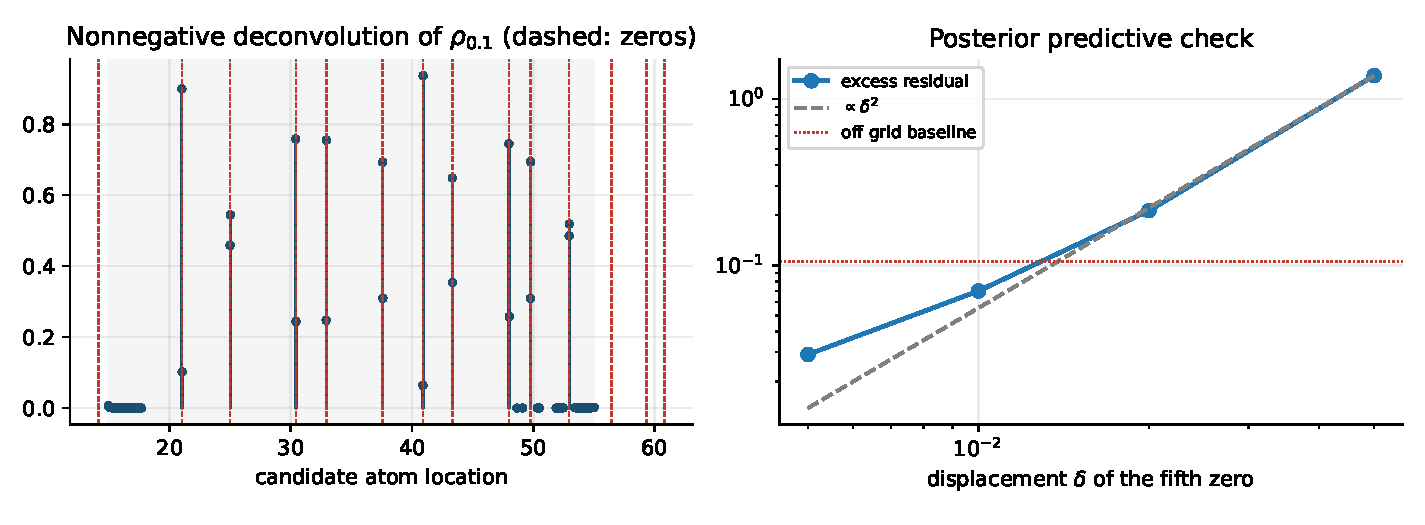
\includegraphics[width=0.95\textwidth]{fig/deconv.pdf}
\caption{Left: the weights of the nonnegative solution for $\rho_{0.1}$ (stems) and the zeros (dashed), with the data window $[15,55]$ shaded. Each zero in the data window carries adjacent weights of total mass one to within half a per cent; the zeros at $14.13$, $56.45$, $59.35$ and $60.83$, outside it, carry none. Right: the excess residual against the displacement $\delta$ of the fifth zero, the $\delta^2$ law through the point at $\delta=0.05$, and the off grid baseline $r_0=0.106$.}
\label{fig:ch17:deconv}
\end{figure}

\subsection{A displaced zero and the threshold of detection}\label{sec:ch17:ppc}

To calibrate the check we displaced the fifth zero, $\gamma_5=32.935$, in the sense of Proposition~\ref{prop:signature}(i): we added to the data the change per displaced zero, $g=\frac12(P_{\varepsilon+\delta}+P_{\varepsilon-\delta})-P_\varepsilon$, centred at $\gamma_5$, and refitted. Twice $g$ is the change in the density when a double zero at $\frac12+i\gamma_5$ leaves the line as the quadruple $\frac12\pm\delta\pm i\gamma_5$, as at a collision in the de Bruijn Newman flow (Section~\ref{ch:dbn}). Table~\ref{tab:ch17:ppc} gives the residuals.

\begin{table}[htbp]
\centering\small
\begin{tabular}{rrrr}
\toprule
$\delta$ & residual $r=\|Aw-y\|$ & excess over baseline & total mass\\
\midrule
0 & 0.1058 & 0 & 10.0942\\
0.005 & 0.1098 & 0.029 & 10.0947\\
0.01 & 0.1269 & 0.070 & 10.0963\\
0.02 & 0.2380 & 0.213 & 10.1031\\
0.05 & 1.3891 & 1.385 & 10.1566\\
\bottomrule
\end{tabular}
\caption{Nonnegative deconvolution of $\rho_{0.1}$ with the signature $g$ of a displaced fifth zero added to the data. Here $r$ is the residual norm and $r_0=0.1058$ its value at $\delta=0$; the excess is $\sqrt{r^2-r_0^2}$.}
\label{tab:ch17:ppc}
\end{table}

For $\delta\ge0.02$ the excess residual grows roughly like $\delta^2$, as the signature does (Proposition~\ref{prop:signature}(i) and \cite[Proposition 19.7]{P26}): it rises from $0.21$ at $\delta=0.02$ to $1.39$ at $\delta=0.05$, a factor $6.5$ for a factor $2.5$ in $\delta$, against $2.5^2=6.25$. At the smallest displacements it grows more slowly, by a factor $2.4$ from $\delta=0.005$ to $0.01$, because there it is dominated by the cross term between the signature and the off grid misfit at $\gamma_5$, which has the same shape. The off grid baseline therefore limits detection: the excess reaches it between $\delta=0.01$ and $0.02$ (Figure~\ref{fig:ch17:deconv}, right). This is the square root law that \eqref{eq:ch8:threshold} states for the matched distance (Section~\ref{sec:ch8:calibration}): since the misfit grows like the square of the displacement, the smallest detectable displacement falls like the square root of the achievable residual, whatever limits the residual. A finer grid of spacing $h$ lowers the baseline like $h^2$ and hence the threshold like $h$, and continuous atom positions would remove the baseline and leave the threshold to the accuracy of the data.

For $\delta\ge\varepsilon$ the check is unreliable. At $\delta=\varepsilon$ the zero $\frac12+\delta+i\gamma_5$ lies on the line of evaluation, where its kernel is a point mass that the samples miss, and the residual, $0.099$, falls below the baseline. For $\delta>\varepsilon$ the atom at $\gamma_5$ leaves the data and is replaced by the signed term $\frac12(P_{\varepsilon+\delta}+P_{\varepsilon-\delta})$ of total mass zero, whose negative part, of mass $\varepsilon/(\pi\delta)+O(\varepsilon^3/\delta^3)$ by Proposition~\ref{prop:signature}(iii), fades as $\delta$ grows. The unit of mass that leaves the data is what the zero density identity of Proposition~\ref{prop:zerodensity} counts, and zeros farther from the line than $\varepsilon$ are left to that identity.

As \cite[Section 19.3.7]{P26} emphasises, this is a model check at finite height and not a route to a proof. What the P\'olya route adds is the small resolution, where the signature $(\delta/\varepsilon)^2$ of Proposition~\ref{prop:signature}(i) is largest for a given $\delta$. The recovery and the calibration are computed, at one resolution and on one window.

The direction of this section is the hard one: Poisson smoothing, which moves the basepoint to the right, preserves positivity, while deconvolution, which moves it back towards the critical line, does not (Section~\ref{ag:sec:exactly}). Chapter~\ref{chap:basepoint} starts instead at the basepoint one, the resolution $\varepsilon=\frac12$ (Section~\ref{ch:basepoint}). At the basepoints between one and the centre, Section~\ref{ch:almost} bounds the mass of the negative part of the split \eqref{ag:eq:split}, the Cauchy kernels of any zeros to the right of the basepoint (Theorem~\ref{ag:thm:almost}), and inserts hypothetical off line zeros into the computed density as this section displaced a zero (Section~\ref{ag:sec:num}).
